%%% Local Variables:
%%% LaTeX-command: "pdflatex --shell-escape"
%%% End:

\documentclass[11pt]{article}
\usepackage[utf8]{inputenc}
\usepackage[T1]{fontenc}
\usepackage{graphicx}
\usepackage{grffile}
\usepackage{longtable}
\usepackage{wrapfig}
\usepackage{rotating}
\usepackage[normalem]{ulem}
\usepackage{amsmath}
\usepackage{textcomp}
\usepackage{amssymb}
\usepackage{capt-of}
\usepackage{hyperref}
\hypersetup{colorlinks=true, linkcolor=magenta}
\setlength{\parindent}{0in}
\usepackage[margin=0.8in]{geometry}
\usepackage[english]{babel}
\usepackage{mathtools}
\usepackage{fancyhdr}
\usepackage{sectsty}
\usepackage{engord}
\usepackage{parskip}
\usepackage{minted}
\usepackage{cite}
\usepackage{graphicx}
\usepackage{setspace}
\usepackage[compact]{titlesec}
\usepackage[center]{caption}
\usepackage{placeins}
\usepackage{color}
\usepackage{amsmath}
\usepackage{bm}
\usepackage{minted}
\usepackage{subfigure}
\usepackage{pdfpages}
% \titlespacing*{\subsection}{0pt}{5.5ex}{3.3ex}
% \titlespacing*{\section}{0pt}{5.5ex}{1ex}
\author{Luis Antonio Ortega Andrés\\Antonio Coín Castro}
\date{\today}
\title{Continuous-time stochastic processes\\\medskip
\large Homework 1}
\hypersetup{
 pdfauthor={Luis Antonio Ortega Andrés},
 pdftitle={Ejercicios de clase},
 pdfkeywords={},
 pdfsubject={},
 pdflang={Spanish}}

% \usemintedstyle{bw}

\begin{document}

\maketitle


\textbf{Exercise 1. }\emph{A Poisson process with rate \( \lambda \) can be defined as a counting process \( \{N(t);\, t \geq 0\} \) with the following properties:}
\begin{enumerate}
  \item \emph{\( N(0) = 0 \) }
  \item \( N(t) \) \emph{has independent and stationary increments}.
  \item \emph{Let \( \Delta N(t)  = N(t + \Delta t) - N(t)\). The following relations hold: }
        \[
        \begin{aligned}
          P[\Delta N(t) = 0] &= 1 - \lambda \Delta t + o(\Delta t),\\
          P[\Delta N(t) = 1] &= \lambda \Delta t + o(\Delta t),\\
          P[\Delta N(t) \geq 2] &= o(\Delta t).\\
        \end{aligned}
        \]
\end{enumerate}
\emph{From this definition show that}
\begin{equation}\label{eq:1}
  P[N(t) = n] = \frac{1}{n!}\lambda^{n}t^{n} e^{-\lambda t}.
\end{equation}

\emph{To this end, set up a system of differential equations for the quantities \( P[N(t) = 0] \) and \( P[N(t) = n] \) with \( n \geq 1 \). Then verify that Equation~\ref{eq:1} satisfies the differential equations derived.}

\emph{Illustrate the validity of the derivation by comparing the empirical distribution obtained in a simulation of the Poisson process and the theoretical distribution of \( P[N(t) = n ]\) given by Equation~\ref{eq:1} for the values \( \lambda = 10 \) and \( t = 2 \).}

\emph{Solution. }For instance, the differential equation for \( P[N(t) = 0]\) can be derived from the fact that
\[
  \begin{aligned}
    P[N(t + \Delta t) = 0] &= P[N(t) = 0]P[\Delta N(t) = 0]\\
    &= P[N(t) = 0](1- \lambda\Delta t + o(\Delta t))\\
    &= P[N(t) = 0] - P[N(t) = 0]\lambda\Delta t + o(\Delta t).
    \end{aligned}
  \]
  Passing \( P[N(t) = 0] \) to the left and dividing in both sides by \( \Delta t \),
  \[
    \frac{P[N(t + \Delta t) = 0] - P[N(t) = 0]}{\Delta t} = - \lambda P[N(t) = 0].
  \]
  Where the following property of \( o(\cdot) \) is used:
  \[
    \lim_{\Delta t \to 0^{+}}\frac{o(\Delta t)}{\Delta t} = 0
  \]
The corresponding differential equation is obtained in the limit \( \Delta t \to 0^{+} \)
\[
  \frac{d}{dt}P[N(t) = 0] = -\lambda P[N(t) = 0].
\]
The solution is this differential equation with initial condition \( P[N(0) = 0] = 1 \) is
\[
  P[N(t) = 0] = e^{-\lambda t}.
\]
Now, given a fixed \( n \geq 1 \), \(  P[N(t + \Delta t) = n] \) can be split into three different successes:
\begin{enumerate}
  \item There is no increment in \( \Delta t \): \(  P[N(t) = n] \) and \(P[\Delta N(t) = 0]\).
  \item There is one increment in \( Delta t \): \(P[N(t) = n-1]\) and \(P[\Delta N(t) = 1] \)
\item There is more than 1 increment in \( \Delta t \): \(  P[N(t + \Delta t) = n]\) and \(P[\Delta N(t) \geq 2] \).
\end{enumerate}
Thus,
\[
  \begin{aligned}
    P[N(t + \Delta t) = n] &= P[N(t) = n]P[\Delta N(t) = 0]\\
    &\ + P[N(t) = n-1]P[\Delta N(t) = 1] \\
    &\ + P[N(t + \Delta t) = n]P[\Delta N(t) \geq 2]\\
    \end{aligned}
  \]
  Where the last term is \( o(\Delta t) \), following the same procedure done before:
  \[
    \frac{P[N(t + \Delta t) = n] - P[N(t) = n]}{\Delta t} = -\lambda P[N(t) = n] + \lambda P([N(t) = n-1]) + \frac{o(\Delta t)}{\Delta t}
  \]
  Limiting in \( \Delta t \to 0^{+} \):
  \[
    \frac{d}{dt}P[N(t) = n] =  -\lambda P[N(t) = n] + \lambda P([N(t) = n-1])
  \]
  Multiplying by \( e^{\lambda t} \)
\[
  e^{\lambda t}\left( \frac{d}{dt}P[N(t) = n]- + \lambda P[N(t) = n] \right) = e^{\lambda t}\lambda P([N(t) = n-1])
\]
\[
  \downarrow
\]
\[
  \frac{d}{dt} e^{\lambda t}P[N(t) = n] = e^{\lambda t}\lambda P([N(t) = n-1]).
\]
Evaluating in \( n = 1 \) and using that \(  P([N(t) = 0]) = e^{-\lambda t}  \)
\[
   \frac{d}{dt} e^{\lambda t}P[N(t) = 1] = e^{\lambda t}\lambda P([N(t) = 0]) = \lambda e^{-\lambda t}e^{\lambda t} = \lambda.
 \]
 Using an inductive procedure, and supposing that \( P[N(t) = n-1] = \frac{1}{(n-1)!}\lambda^{n-1}t^{n-1} e^{-\lambda t} \).
 \[
    \frac{d}{dt} e^{\lambda t}P[N(t) = n] = e^{\lambda t}\lambda P([N(t) = n-1]) = \frac{\lambda}{(n-1)!}\lambda^{n-1}t^{n-1}
 \]
\[
  e^{\lambda t}P[N(t) = n] = \frac{1}{n!}\lambda^{n}t^{n} + c.
\]
Where \( c = 0 \) given that \( P[N(t) = n] = 0\).
\newpage


\textbf{Exercise 2. }\emph{Simulate a Poisson process with \( \lambda = 5.0 \). From these simulations show for different values of \( n = 1,2,5 \) and \( 10 \) that the probability density of the \( n^{th} \) arrival is  }
\begin{equation}
  \label{eq:erlang}
  f_{S_{n}}(t) = \frac{1}{(n-1)!} \lambda^{n}t^{n-1}e^{-\lambda t}.
\end{equation}

\textit{Solution.} We simulate $10000$ Poisson processes with rate $\lambda = 5$, using the code available in the file \verb|src/arrival.py|. From these simulations we extract the times of the first, second, fifth and tenth events, and we create a histogram of them. We also depict the estimated kernel density, and the true density of these arrival times. We know that the $n$th arrival time follows an Erlang distribution with shape parameter $n$ and rate $\lambda$, whose p.d.f is given by Eq. \eqref{eq:erlang}}. After running \verb|src/2.py| we obtain the following graphs:

\begin{figure}[h!]
  \centering
  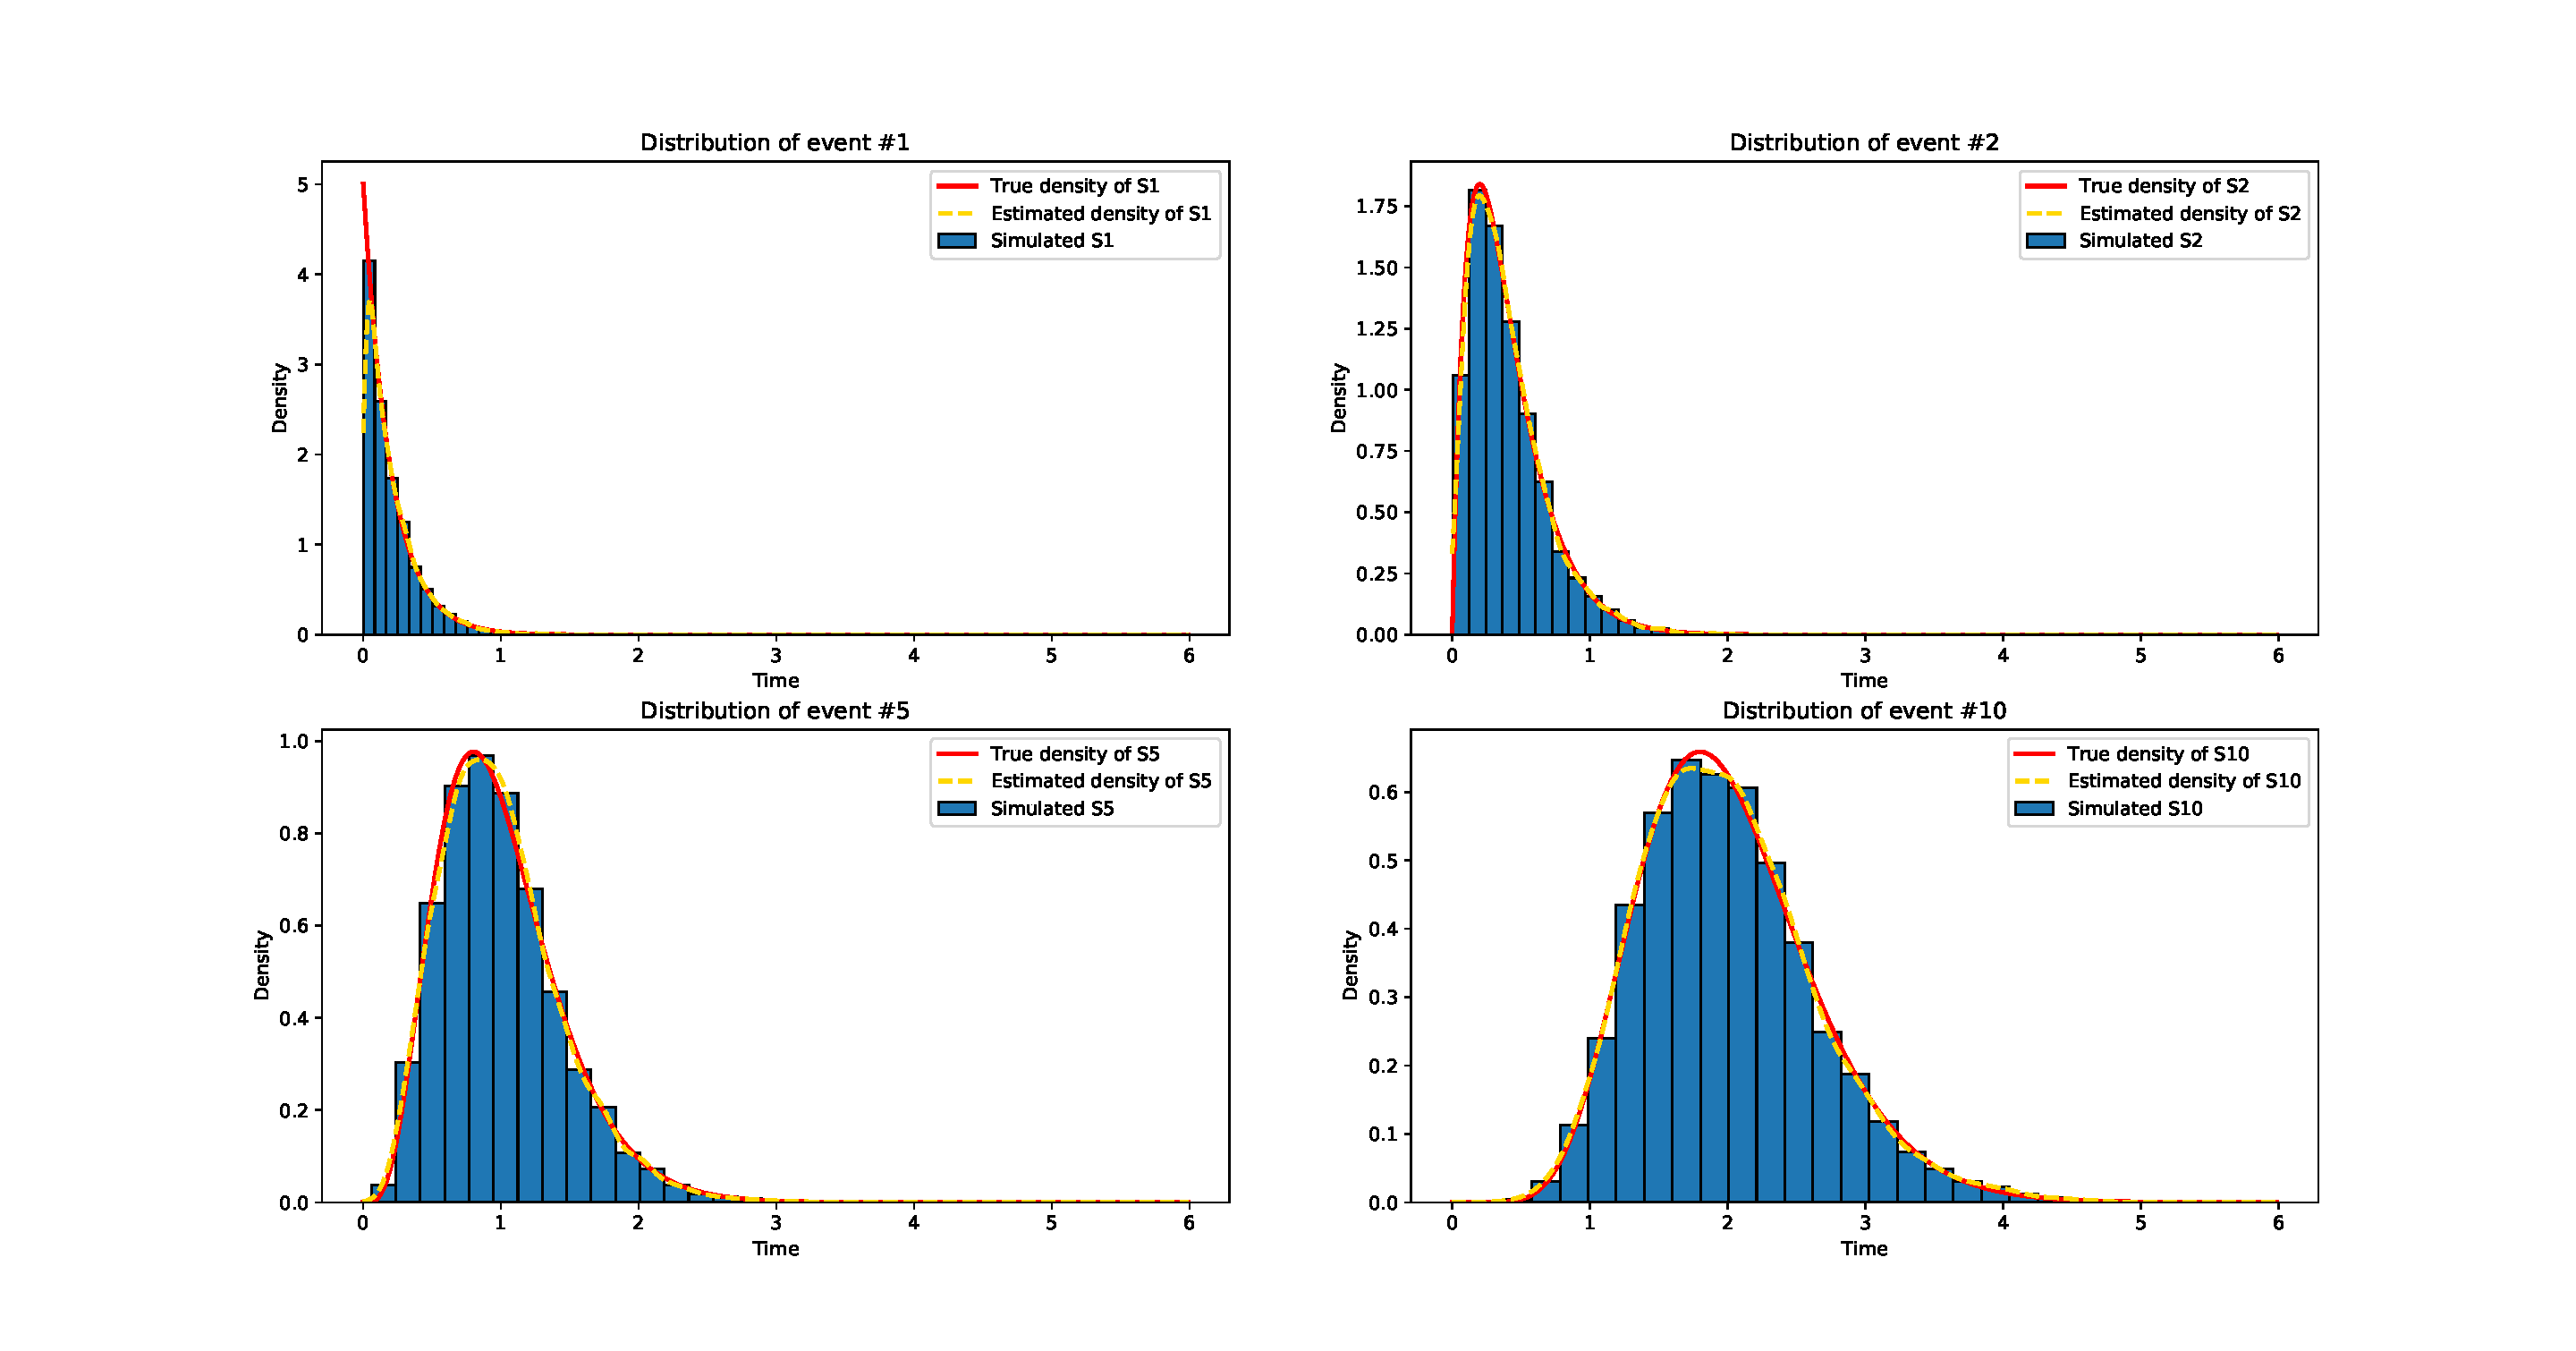
\includegraphics[width=\textwidth]{img/ex2.pdf}
\end{figure}

As we can see, the simulations agree with the theoretical distribution for each arrival time.\\


\textbf{Exercise 3. }\emph{Assume that we have a sample \( \{U_{i}\}_{i=1,\dots,n} \) of \( n \) i.i.d  \(U_{i} \sim U[0, t] \) random variables. The probability density of the order statistics \( \{U_{(1)} < U_{(2)} < \cdots < U_{(n)}\} \)  is}
\[
  f_{U_{(1)},\dots,U_{(n)}}(u_{(1)},\dots,u_{(n)}) = \frac{n!}{t^{n}}.
\]

\emph{Let \( \{N(t): \, t \geq 0\} \) be a Poisson process with rate \( \lambda \). show that conditioned on \( N(t) = n \), the distribution of the arrival times \( \{0 < S_{1} < S_{2} < \dots < S_{n}\} \) coincides with the distribution of order statistics of \( n \) i.i.d \( U[0, t] \) random variables, i.e.:}
\[
  f_{S_{1},\dots,S_{n} \mid N(t)}(s_{1},\dots, s_{n} \mid N(t) = n) = \frac{n!}{t^{n}}.
\]

\emph{Solution.} Consider a fixed sample $\{s_1, \dots, s_n\}$ of arrival times, where necessarily $t\geq s_n$. From now on, we will drop the subindexes when possible to avoid cluttering the notation, and we will use ``$f$'' to represent both a p.d.f. and a p.m.f. interchangeably. We split up the proof in several steps.

Firstly, using Bayes' theorem we have:
\begin{equation}
  \label{eq:bayes}
  f(s_{1},\dots, s_{n+1} \mid N(t) = n) = \frac{ f(N(t) = n \mid s_{1},\dots, s_{n+1}) f(s_{1},\dots, s_{n+1})  }{ f(N(t) = n)  }.
\end{equation}
Now we may use the self-evident fact that \( N(t) = n \iff s_{n} \leq t < s_{n+1} \) in order to write
\[
  f(N(t) = n \mid s_{1},\dots, s_{n+1}) = \begin{cases} 1 & s_{n} \leq t < s_{n+1}\\ 0 &\text{otherwise} \end{cases}.
\]
From this distinction and looking at Eq. \eqref{eq:bayes} it follows that
\[
   f(s_{1},\dots,s_{n+1} \mid N(t) = n) \neq 0 \iff s_{n} \leq t < s_{n+1},
 \]
 which makes perfect sense: \emph{the probability of observing $n+1$ events at times $s_1, \dots, s_{n+1}$, having observed $n$ events at time $t$, is positive if and only if the $n$ events were observed just at or after the second-to-last arrival time and strictly before the last one.}

For this reason we will be focusing on the case \(s_{n} \leq t < s_{n+1} \), in which Eq. \eqref{eq:bayes} translates to\footnote{The expression for $f(s_1,\dots,s_{n+1})$ can be derived from the fact that the time increments $T_i=S_{i}-S_{i-1}$ are identically (exponentially) distributed and independent: $f(s_1,\dots,s_{n+1})=f(T_1=s_1)f(T_2=s_2-s_1)\cdots f(T_{n+1}=s_{n+1}-s_n)$.}
 \begin{equation}
   \label{eq:aux3}
    f(s_{1},\dots, s_{n+1} \mid N(t) = n) = \frac{ f(s_{1},\dots, s_{n+1})  }{ f(N(t) = n)  } = \dfrac{\lambda ^{n+1} \exp(-\lambda s_{n+1})}{\frac{1}{n!} (\lambda t)^{n} \exp (- \lambda t)} = \frac{n! \lambda \exp(-\lambda (s_{n+1}-t))}{t^{n}}.
 \end{equation}
Next, we will use the fact that the conditional probability factorizes as:
\[
  f(s_{1},\dots,s_{n+1} \mid N(t)=n) = f(s_{n+1} \mid s_{1},\dots, s_{n}, N(t)=n)f(s_{1},\dots,s_{n}\mid N(t)=n),
\]
and also the \emph{memoryless} property for \( s_{n+1} > t \):
\[
  f(s_{n+1} \mid s_{1},\dots, s_{n}, N(t)=n) = f(s_{n+1} \mid N(t)=n).
\]

Combining these two properties, we have:
\[
f(s_1,\dots, s_n \mid N(t)=n) = \frac{f(s_1,\dots, s_{n+1} \mid N(t)=n)}{f(s_{n+1}\mid N(t)=n)}.
\]
The numerator in the RHS of the previous expression is given by Eq. \eqref{eq:aux3}}. The denominator can be comptued if we realize that, conditional on $N(t)=n$, the time instant $s_{n+1}$ is the \textit{first arrival time after time $t$}. In other words, it follows the same distribution as the first arrival time if the origin had been put at time $t$, whichs is an \textit{Erlang}$(1,\lambda)$ shifted by the location parameter $t$. Putting it all together we arrive at the desired result:
\[
  f(s_{1},\dots,s_{n}\mid N(t)=n) = \frac{n!}{t^{n}} \frac{\lambda\exp(-\lambda (s_{n+1}-t))}{\lambda\exp(-\lambda (s_{n+1}-t))} = \frac{n!}{t^{n}}.
\]\hfill $\square$\\


\textbf{Exercise 4. }\emph{Two teams A and B play a soccer match. The number of goals scored by Team A is modeled by a Poisson process \( N_{1}(t) \) with rate \( \lambda_{1} = 0.02 \) goals per minute. The number of goals scored by Team B is modeled by a Poisson process \( N_{2}(t)\) with rate \( \lambda_{2} = 0.03\) goals per minute. The two processes are assumed to be independent. Let \( N(t) \) be the total number of goals in the game up to and including time \( t \). The game lasts for \( 90 \) minutes.}
\begin{enumerate}
  \item[\textit{(i)}] \emph{Find the probability that no goals are scored}.
  \item[\textit{(ii)}] \emph{Find the probability that at least two goals are scored in the game.}
  \item[\textit{(iii)}] \emph{Find the probability of the final score being Team A: 1, Team B: 2.}
  \item[\textit{(iv)}]  \emph{Find the probability that they draw}.
  \item[\textit{(v)}]  \emph{Find the probability that Team B scores the first goal}.
\end{enumerate}
\emph{Confirm your results by writing a Python program that simulates the process and estimate the answers from the simulations.}

\emph{Solution.} We know that the sum of two independent Poisson processes is also a Poisson process with rate equal to the sum of the rates, so we can write $N(t)\sim Poisson(0.05)$. We will make repeated use of the expression of the p.m.f. of a Poisson process (see Eq. \eqref{eq:1}).
\begin{enumerate}
  \item[\textit{(i)}] The probability that no goals are scored equals:
        \[
        P[N(90) = 0] = \frac{1}{0!}(0.05\cdot 90)^0 e^{-0.05\cdot 90} = e^{-4.5} \approx 0.0111.
        \]
  \item[\textit{(ii)}] The probability that at least two goals are scored in the game is:
        \[
        \begin{aligned}
          P[N(90) \geq 2] &= 1 - P[N(90)\leq 1] = 1 - \left( P[N(90)=0]+P[N(90)=1]\right)\\
          &= 1 - (e^{-4.5} + 0.05 \cdot 90 e^{-4.5}) \approx 0.9389.
        \end{aligned}
        \]
  \item[\textit{(iii)}] Since $N_1(t)$ and $N_2(t)$ are independent, the probability of finishing with a score of Team A: $1$ and Team B: $2$ is:
        \[
        \begin{aligned}
        &P[N_1(90)=1, N_2(90)=2] = P[N_{1}(90) = 1]P[N_{2}(90) = 2]\\
        &= 0.02\cdot 90e^{-0.02 \cdot 90} \frac{1}{2}\cdot 0.03^{2}\cdot 90^{2}e^{-0.03\cdot90} \approx 0.0729.
      \end{aligned}
        \]
  \item[\textit{(iv)}] The probability that they draw is given by the expression:
        \[
        P[N_1(90) = N_2(90)] = \sum_{n=0}^{\infty} P[N_{1}(90) = n]P[N_{2}(90) = n] = \sum_{n=0}^{\infty}\frac{1}{(n!)^{2}}0.02^{n}0.03^{n}90^{2n}e^{-90(0.03 + 0.02)}.
        \]
        We could try to sum this infinite series, but we are better off using the fact that the difference of two independent Poisson variables follows a \href{https://en.wikipedia.org/wiki/Skellam_distribution}{Skellam distribution}. Indeed, if $V_1$ and $V_2$ are two independent Poisson-distributed random variables with means $\lambda_1$ and $\lambda_2$ respectively, the p.m.f. for the difference $V=V_1-V_2$ is given by:
        \begin{equation}\label{eq:skellam}
        p(\nu; \lambda_1, \lambda_2) = P[V=\nu]=e^{-(\lambda_1+\lambda_2)}\left(\frac{\lambda_1}{\lambda_2}\right)^{\nu/2}I_{\nu}(2\sqrt{\lambda_1\lambda_2}),
      \end{equation}
        where $I_\nu(x)$ is the modified Bessel function of the first kind of order \( \nu \), i.e.:
\[
  I_{\nu}(x) = \sum_{n=0}^{\infty} \frac{1}{n! \Gamma(n + \nu + 1)}\left( \frac{x}{2} \right)^{2n + \nu}.
\]
Now we can compute the desired probability with the aid of Python, either by evaluating the p.m.f. of a $Skellam(90\cdot 0.02, 90\cdot 0.03)$ at $\nu=0$ with \verb|scipy.stats.skellam|, or by substituting the appropriate values in Eq. \eqref{eq:skellam} and evaluating $I_0$ in the corresponding point via \verb@scipy.special.iv@. Either way, we have:
\[
P[N_1(90)- N_2(90) = 0]=e^{-90\cdot 0.05}I_0(2\cdot 90\sqrt{0.02\cdot 0.03}) \approx 0.1793.
\]
  \item[\textit{(v)}] Let $X$ model the time of the first goal scored by Team B, and let $Y$ be the number of goals scored by Team A before Team B scores. On the one hand we have that, conditional on $X=t$, the variable $Y$ is counting the number of events (goals of Team A) up to time $t$, so it may be viewed as a Poisson process with mean $0.02t$:
  \[
  P[Y=n\mid X=t]=\frac{1}{n!}(0.02t)^n e^{-0.02t}.
  \]
  On the other hand, the distribution of $X$ is that of the first arrival time of the Poisson process $N_2(t)$, which is known to be exponentially distributed:
  \[
  P[X=t]= 0.03e^{-0.03t}.
  \]
  With this notation, we are interested in computing the probability of $Y=0$, given the restrictions that $0\leq X\leq 90$ (that is, we are requiring that Team B scores at least once). Combining the above expressions and using the \textit{law of total probability}, we get:
  \[
  \begin{aligned}
  &P[Y=0\mid0\leq X \leq 90]=\int_0^{90} P[Y=0\mid X=t]P[X=t]\, dt\\
  &=  \int_0^{90}0.03 e^{-0.05t}\, dt= -\frac{0.03}{0.05}\Big[ e^{-0.05t}\Big]_0^{90} \approx 0.5933.
\end{aligned}
  \]
\end{enumerate}

The simulations can be seen in the attached notebook.\\

\end{document}
